\PassOptionsToPackage{unicode=true}{hyperref} % options for packages loaded elsewhere
\PassOptionsToPackage{hyphens}{url}
%
\documentclass[12pt,]{article}
\usepackage{lmodern}
\usepackage{amssymb,amsmath}
\usepackage{ifxetex,ifluatex}
\usepackage{fixltx2e} % provides \textsubscript
\ifnum 0\ifxetex 1\fi\ifluatex 1\fi=0 % if pdftex
  \usepackage[T1]{fontenc}
  \usepackage[utf8]{inputenc}
  \usepackage{textcomp} % provides euro and other symbols
\else % if luatex or xelatex
  \usepackage{unicode-math}
  \defaultfontfeatures{Ligatures=TeX,Scale=MatchLowercase}
\fi
% use upquote if available, for straight quotes in verbatim environments
\IfFileExists{upquote.sty}{\usepackage{upquote}}{}
% use microtype if available
\IfFileExists{microtype.sty}{%
\usepackage[]{microtype}
\UseMicrotypeSet[protrusion]{basicmath} % disable protrusion for tt fonts
}{}
\IfFileExists{parskip.sty}{%
\usepackage{parskip}
}{% else
\setlength{\parindent}{0pt}
\setlength{\parskip}{6pt plus 2pt minus 1pt}
}
\usepackage{hyperref}
\hypersetup{
            pdftitle={Supplementary material},
            pdfborder={0 0 0},
            breaklinks=true}
\urlstyle{same}  % don't use monospace font for urls
\usepackage[margin=1.0in]{geometry}
\usepackage{graphicx,grffile}
\makeatletter
\def\maxwidth{\ifdim\Gin@nat@width>\linewidth\linewidth\else\Gin@nat@width\fi}
\def\maxheight{\ifdim\Gin@nat@height>\textheight\textheight\else\Gin@nat@height\fi}
\makeatother
% Scale images if necessary, so that they will not overflow the page
% margins by default, and it is still possible to overwrite the defaults
% using explicit options in \includegraphics[width, height, ...]{}
\setkeys{Gin}{width=\maxwidth,height=\maxheight,keepaspectratio}
\setlength{\emergencystretch}{3em}  % prevent overfull lines
\providecommand{\tightlist}{%
  \setlength{\itemsep}{0pt}\setlength{\parskip}{0pt}}
\setcounter{secnumdepth}{0}
% Redefines (sub)paragraphs to behave more like sections
\ifx\paragraph\undefined\else
\let\oldparagraph\paragraph
\renewcommand{\paragraph}[1]{\oldparagraph{#1}\mbox{}}
\fi
\ifx\subparagraph\undefined\else
\let\oldsubparagraph\subparagraph
\renewcommand{\subparagraph}[1]{\oldsubparagraph{#1}\mbox{}}
\fi

% set default figure placement to htbp
\makeatletter
\def\fps@figure{htbp}
\makeatother

\usepackage{times} % Times New Roman font
\usepackage[T1]{fontenc}

\usepackage[none]{hyphenat}

\usepackage{setspace}
\doublespacing
\setlength{\parskip}{1em}

\usepackage{lineno}
\renewcommand{\linenumberfont}{\normalfont\tiny}

\usepackage{pdfpages}

\usepackage{indentfirst}

\usepackage[labelsep=period, labelfont=bf]{caption}
\renewcommand{\thefigure}{S\arabic{figure}}
\renewcommand{\figurename}{Supplementary Figure}
\renewcommand{\thetable}{S\arabic{table}}
\renewcommand{\tablename}{Supplementary Table}
\captionsetup{justification=raggedright,singlelinecheck=false}

\usepackage{pdflscape}
\newcommand{\blandscape}{\begin{landscape}}
\newcommand{\elandscape}{\end{landscape}}

\usepackage{siunitx}
\DeclareSIUnit\molar{\mole\per\cubic\deci\metre}
\DeclareSIUnit\Molar{\textsc{m}}
\DeclareSIUnit\cells{\text{cells}}

\usepackage{caption}
\captionsetup{justification=justified}

\usepackage{float}

\usepackage{txfonts}

\renewcommand{\figureautorefname}{Figure}

\usepackage{microtype}
\usepackage{etoolbox}
\makeatletter
\providecommand{\subtitle}[1]{% add subtitle to \maketitle
  \apptocmd{\@title}{\par {\large #1 \par}}{}{}
}
\makeatother
\usepackage{booktabs}
\usepackage{longtable}
\usepackage{array}
\usepackage{multirow}
\usepackage{wrapfig}
\usepackage{float}
\usepackage{colortbl}
\usepackage{pdflscape}
\usepackage{tabu}
\usepackage{threeparttable}
\usepackage{threeparttablex}
\usepackage[normalem]{ulem}
\usepackage{makecell}
\usepackage{xcolor}

\title{\textbf{Supplementary material}}
\providecommand{\subtitle}[1]{}
\subtitle{Compositional stability of sediment microbial communities during a
seagrass meadow decline}
\author{}
\date{\vspace{-2.5em}}

\begin{document}
\maketitle

\vspace{10mm}

Marsej Markovski\textsuperscript{1}, Mirjana Najdek\textsuperscript{1},
Gerhard J. Herndl\textsuperscript{2,3}, and Marino
Korlević\textsuperscript{1\(*\)}

1. Center for Marine Research, Ruđer Bošković Institute, Croatia

2. Department of Functional and Evolutionary Ecology, University of
Vienna, Austria

3. Department of Marine Microbiology and Biogeochemistry, Royal
Netherlands Institute for Sea Research (NIOZ), Utrecht University, The
Netherlands

\textsuperscript{\(*\)}To whom correspondence should be addressed:

Marino Korlević

G. Paliaga 5, 52210 Rovinj, Croatia

Tel.: +385 52 804 768

Fax: +385 52 804 780

e-mail:
\href{mailto:marino.korlevic@irb.hr}{\nolinkurl{marino.korlevic@irb.hr}}

Running title: Compositional stability of sediment communities

\sisetup{mode=text}
\setlength\parindent{24pt}

\hypertarget{supplementary-figures}{%
\subsection{Supplementary figures}\label{supplementary-figures}}

\begin{figure}[H]

{\centering 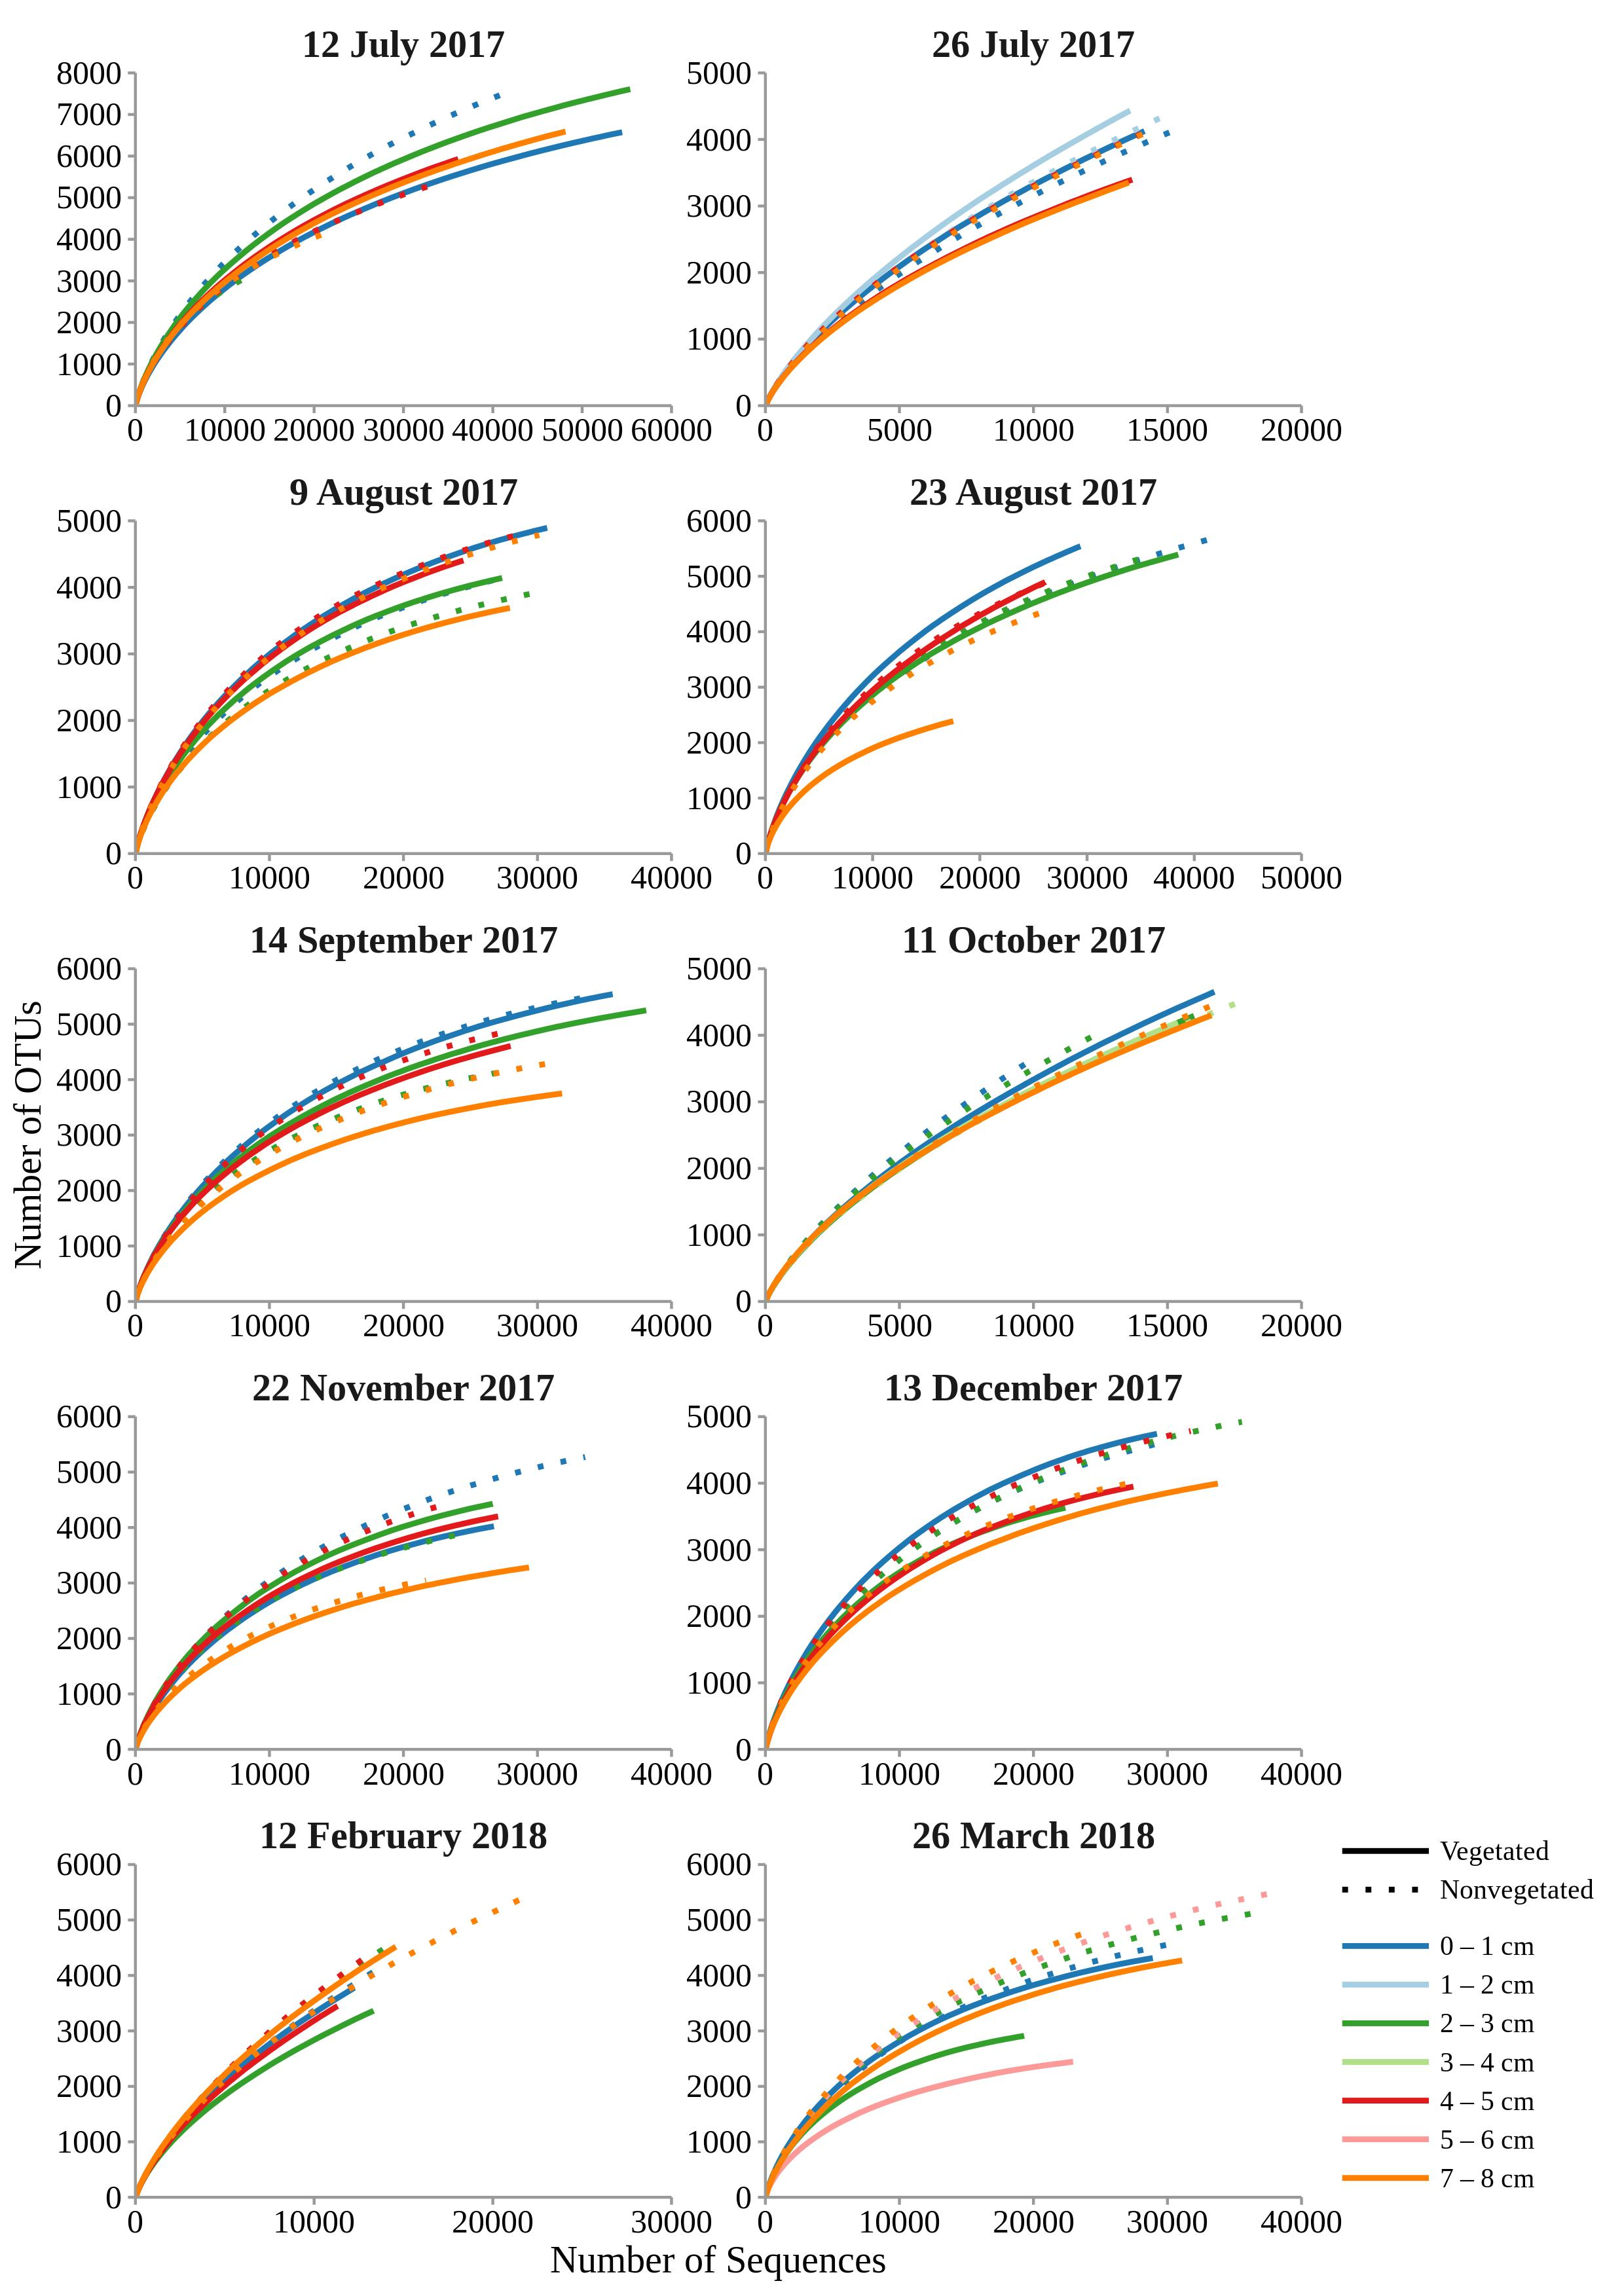
\includegraphics[width=0.85\linewidth]{../results/figures/rarefaction_a} 

}

\caption{Rarefaction curves of sediment microbial communities sampled at the vegetated and nonvegetated site in the Bay of Saline from 12 July 2017 to 26 March 2018.\label{rarefaction_a}}\label{fig:unnamed-chunk-1}
\end{figure}

\begin{figure}[H]

{\centering 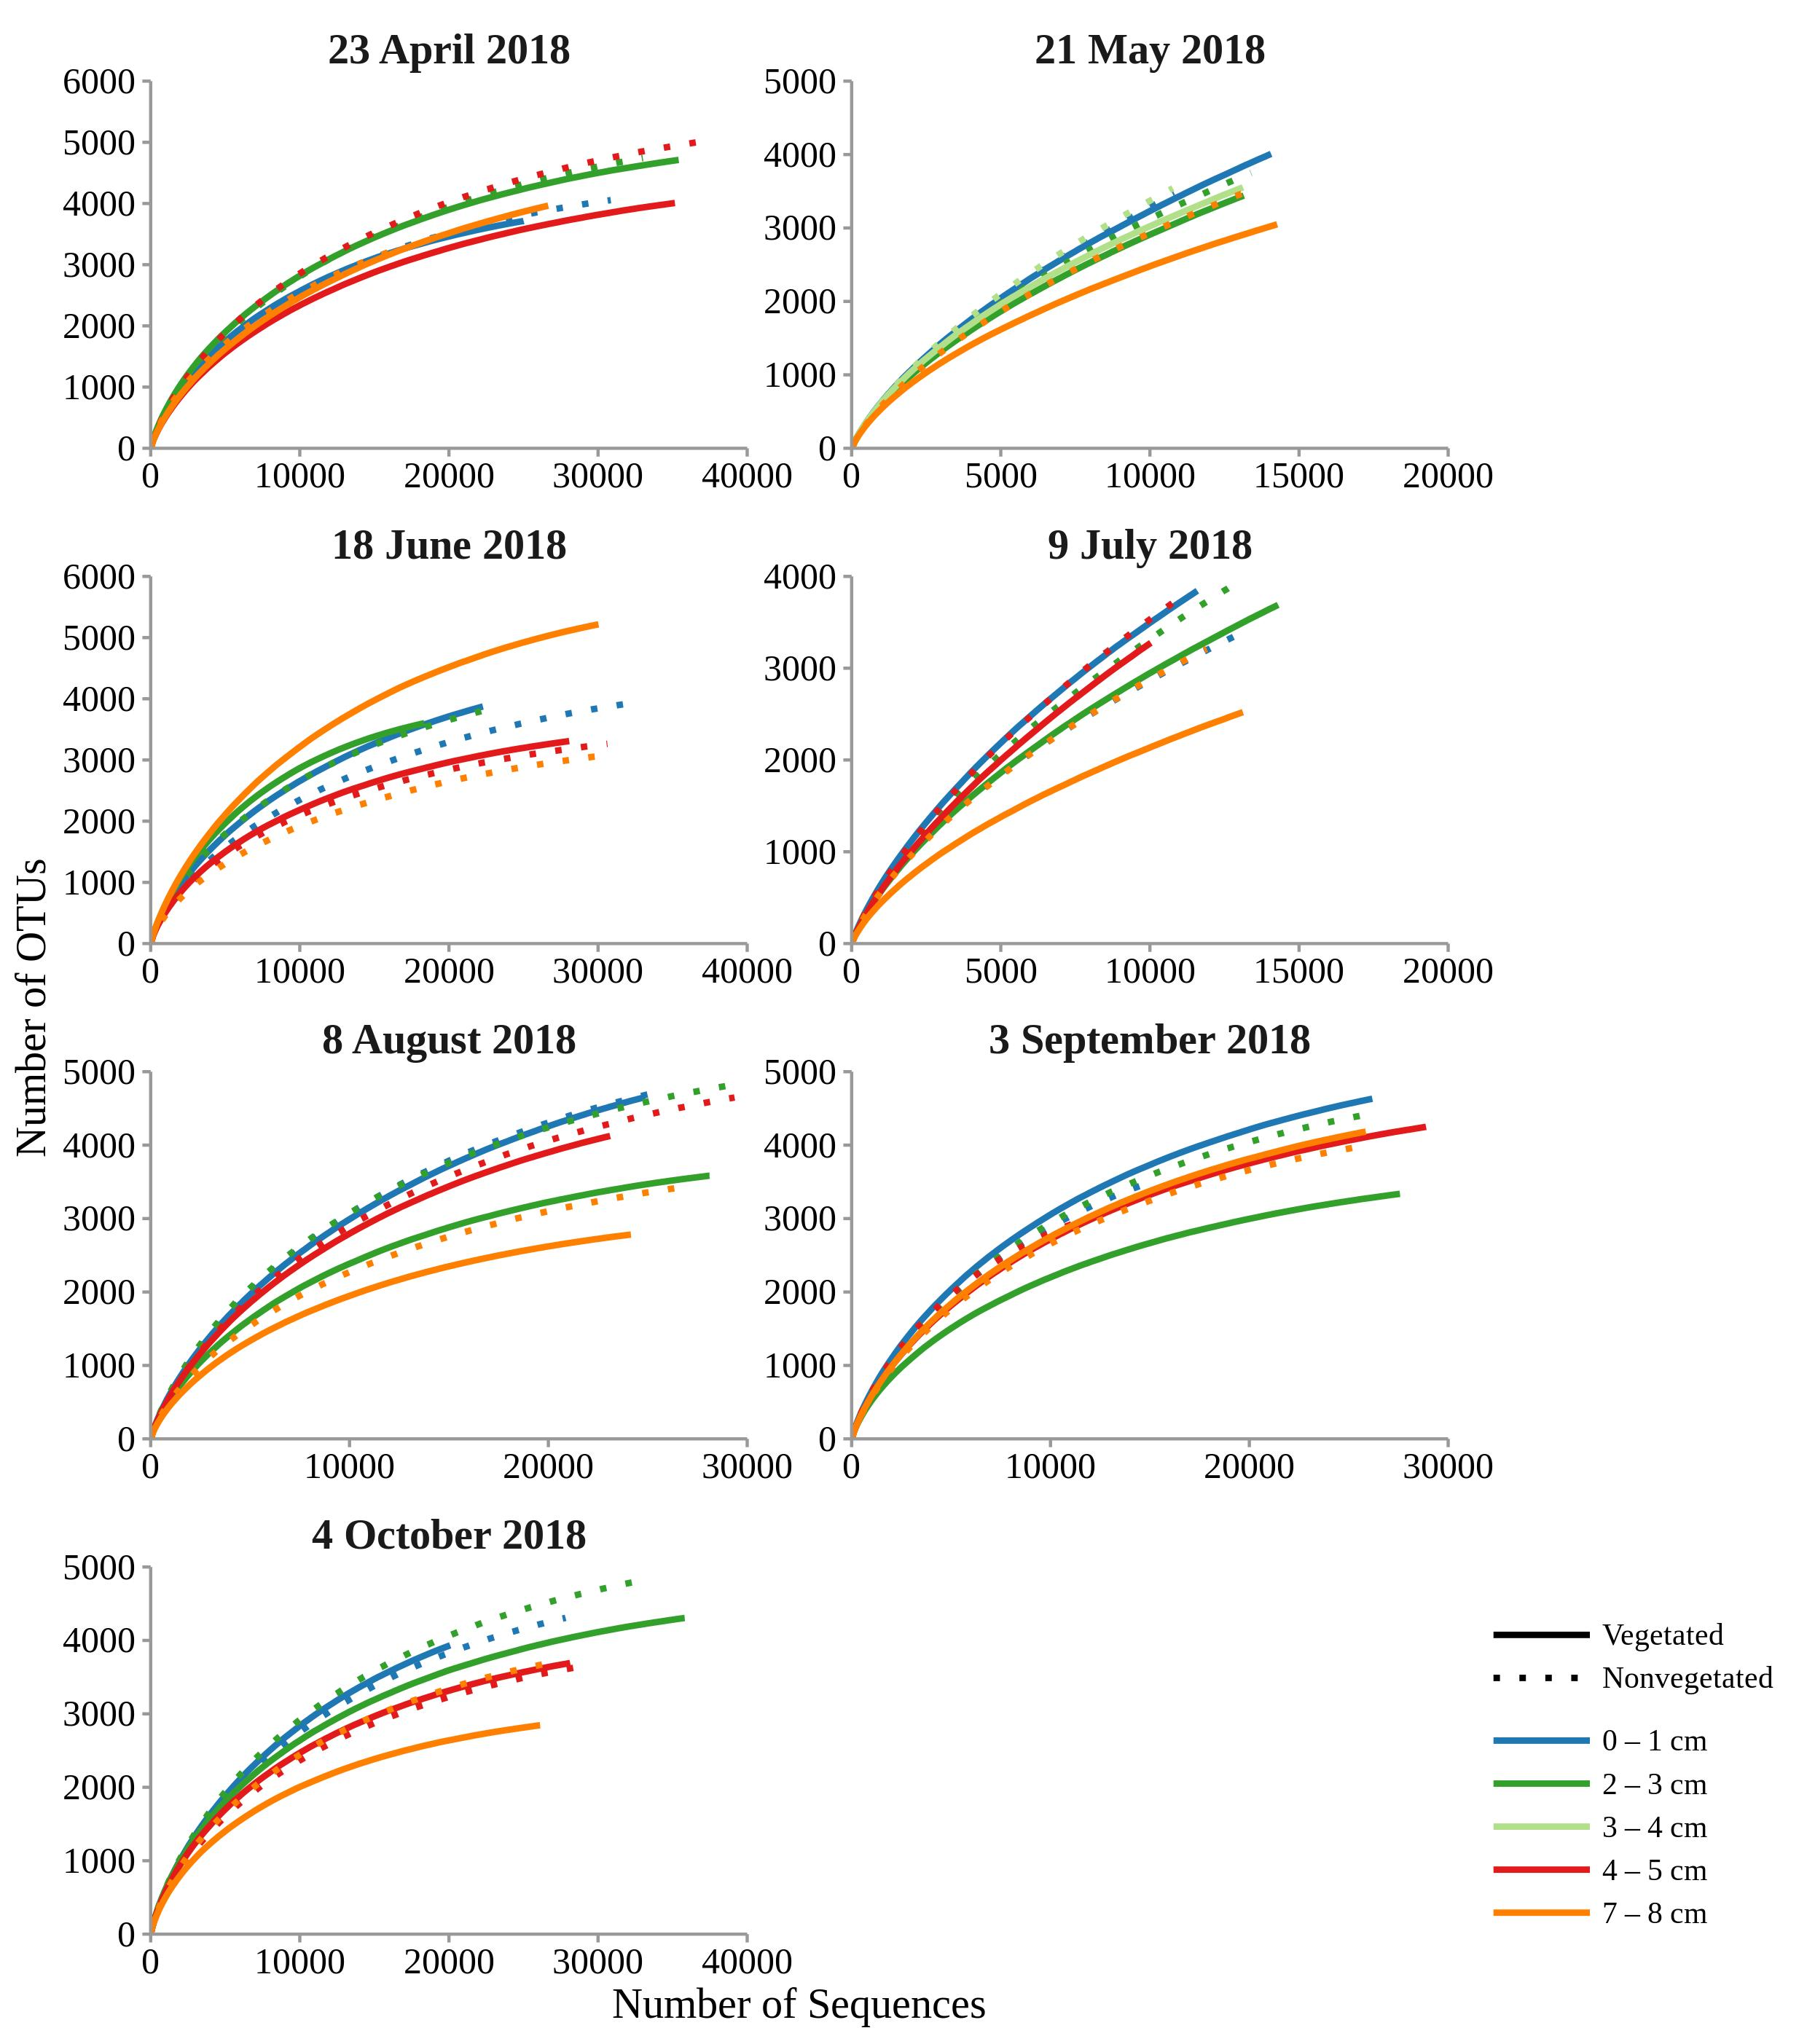
\includegraphics[width=0.85\linewidth,height=0.8\textheight]{../results/figures/rarefaction_b} 

}

\caption{Rarefaction curves of sediment microbial communities sampled at the vegetated and nonvegetated site in the Bay of Saline from 23 April 2018 to 4 October 2018.\label{rarefaction_b}}\label{fig:unnamed-chunk-2}
\end{figure}

\begin{figure}[H]

{\centering 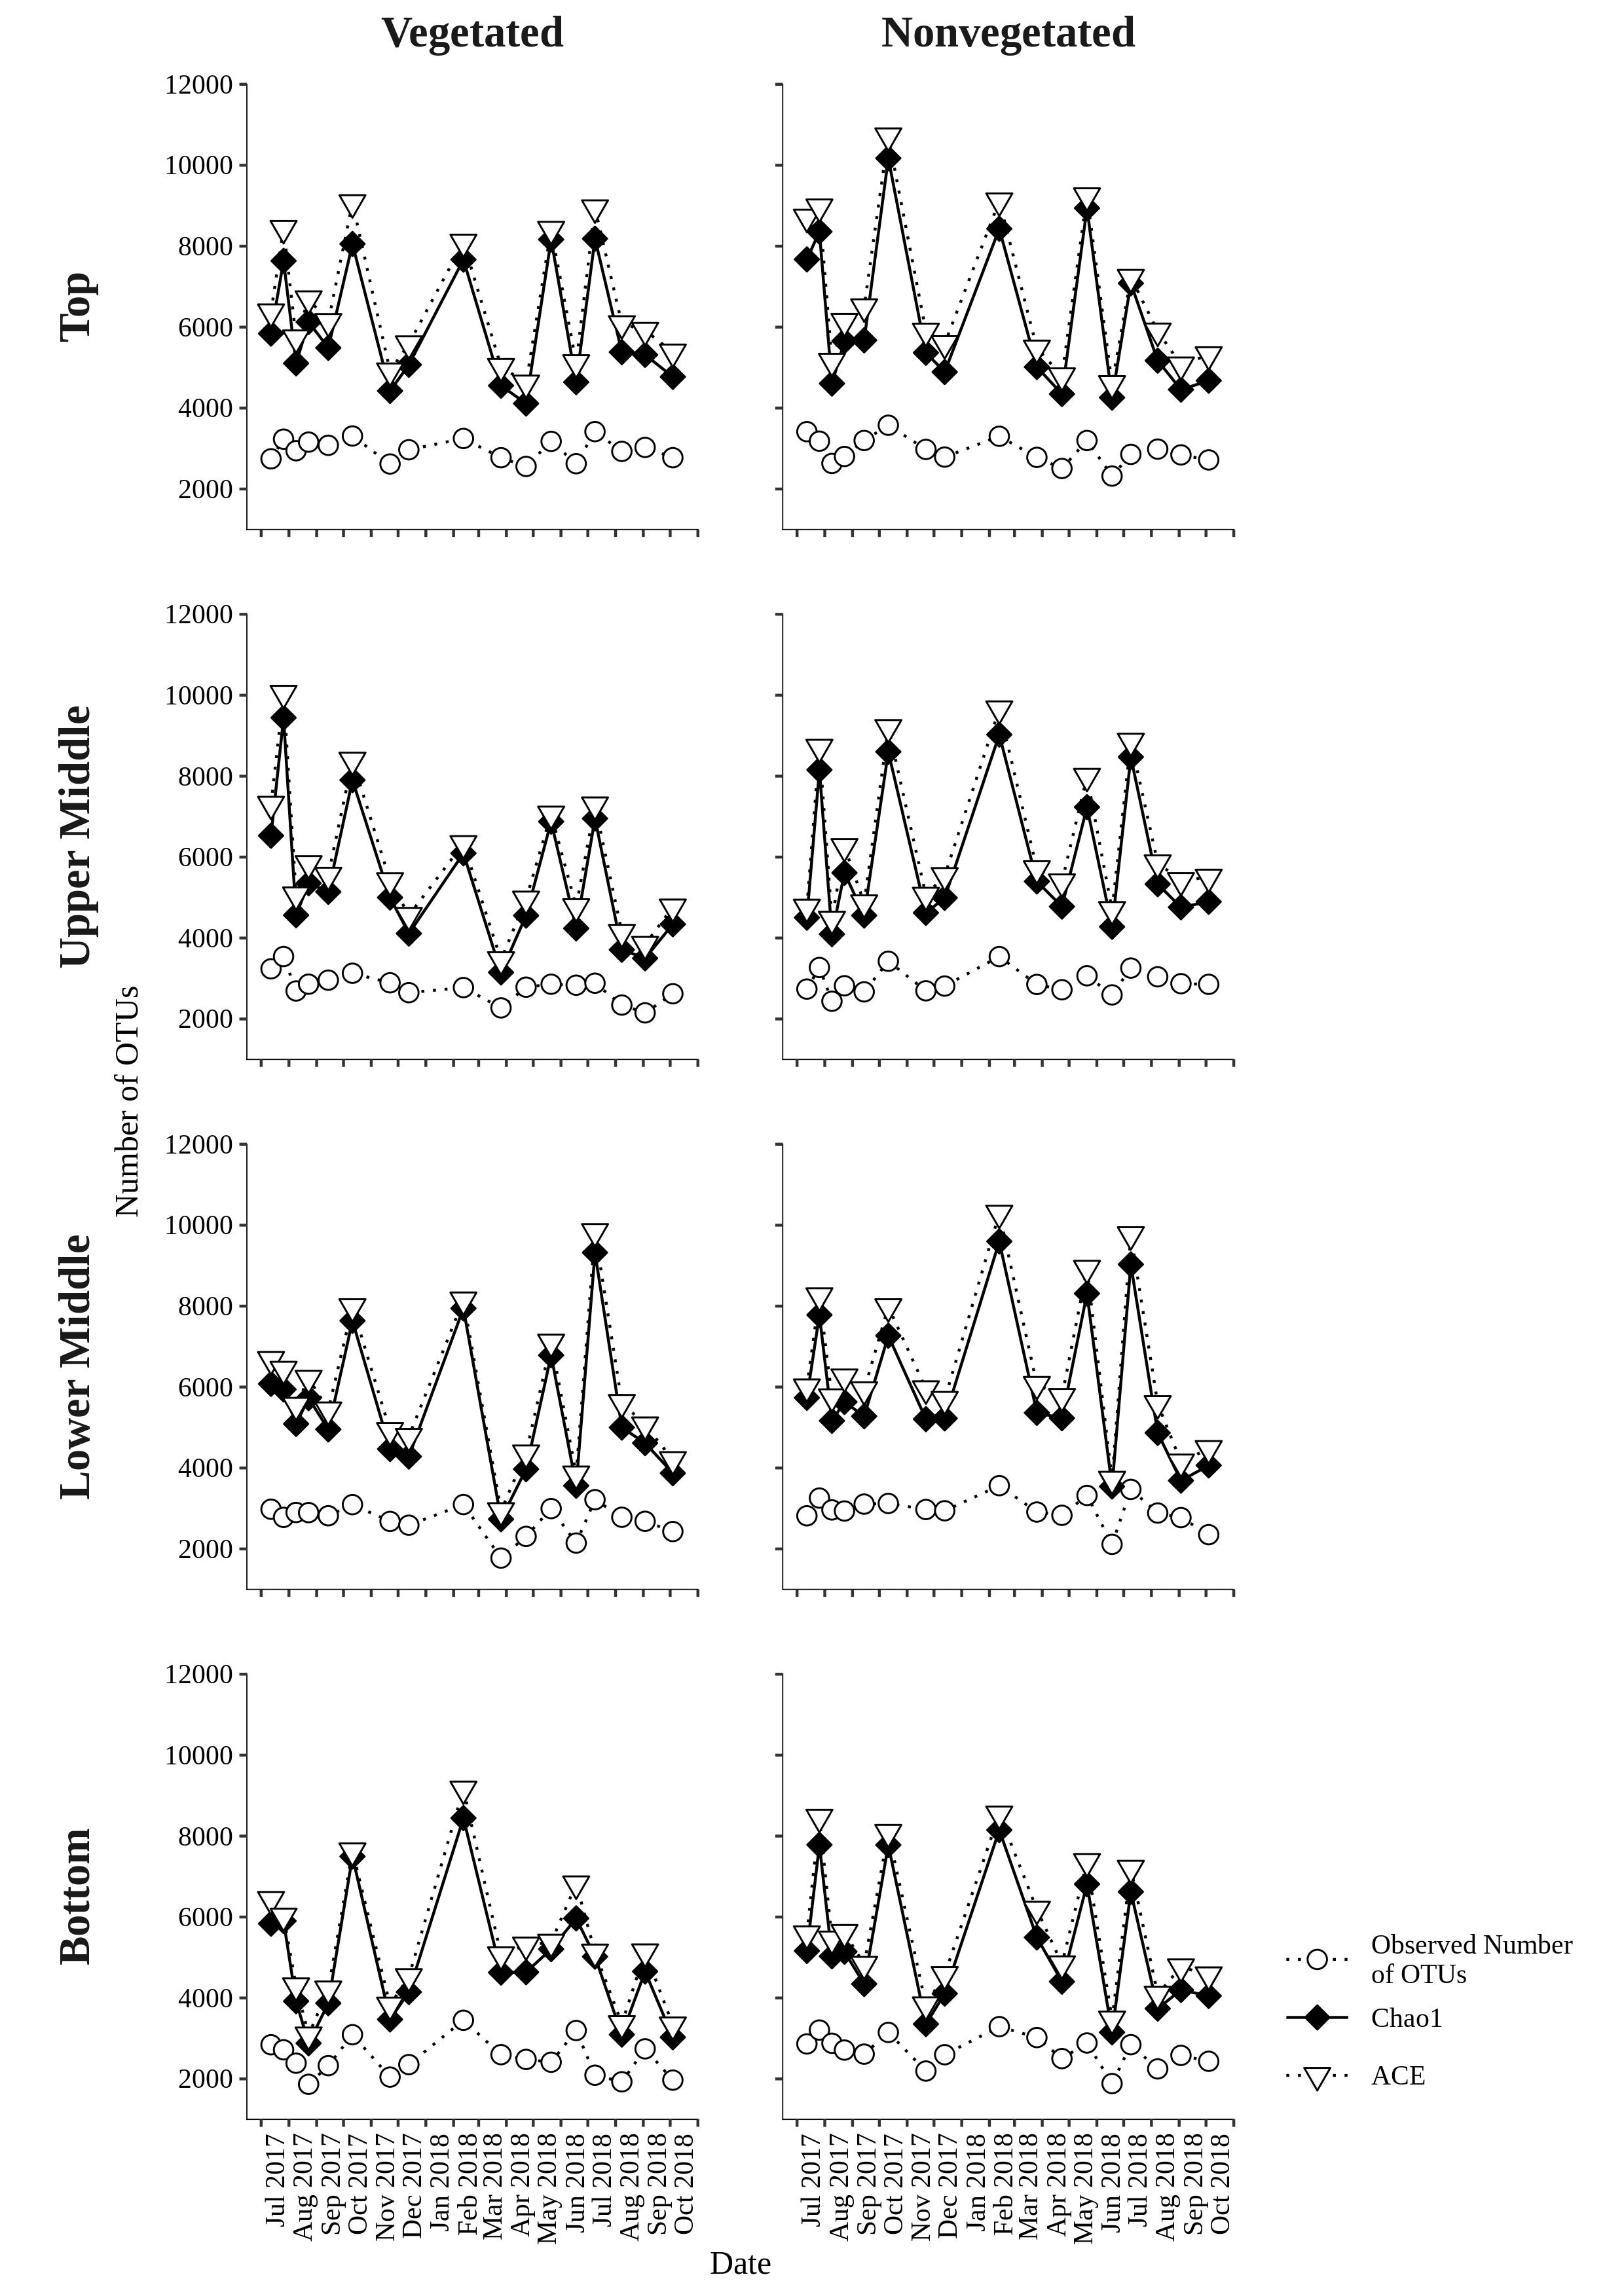
\includegraphics[width=0.9\linewidth,height=1\textheight]{../results/figures/estimators_months} 

}

\caption{Temporal dynamics of the observed number of OTUs, Chao1, and ACE of sediment microbial communities sampled in different sediment layers of the vegetated and nonvegetated site in the Bay of Saline.\label{estimators_moths}}\label{fig:unnamed-chunk-3}
\end{figure}

\begin{figure}[H]

{\centering 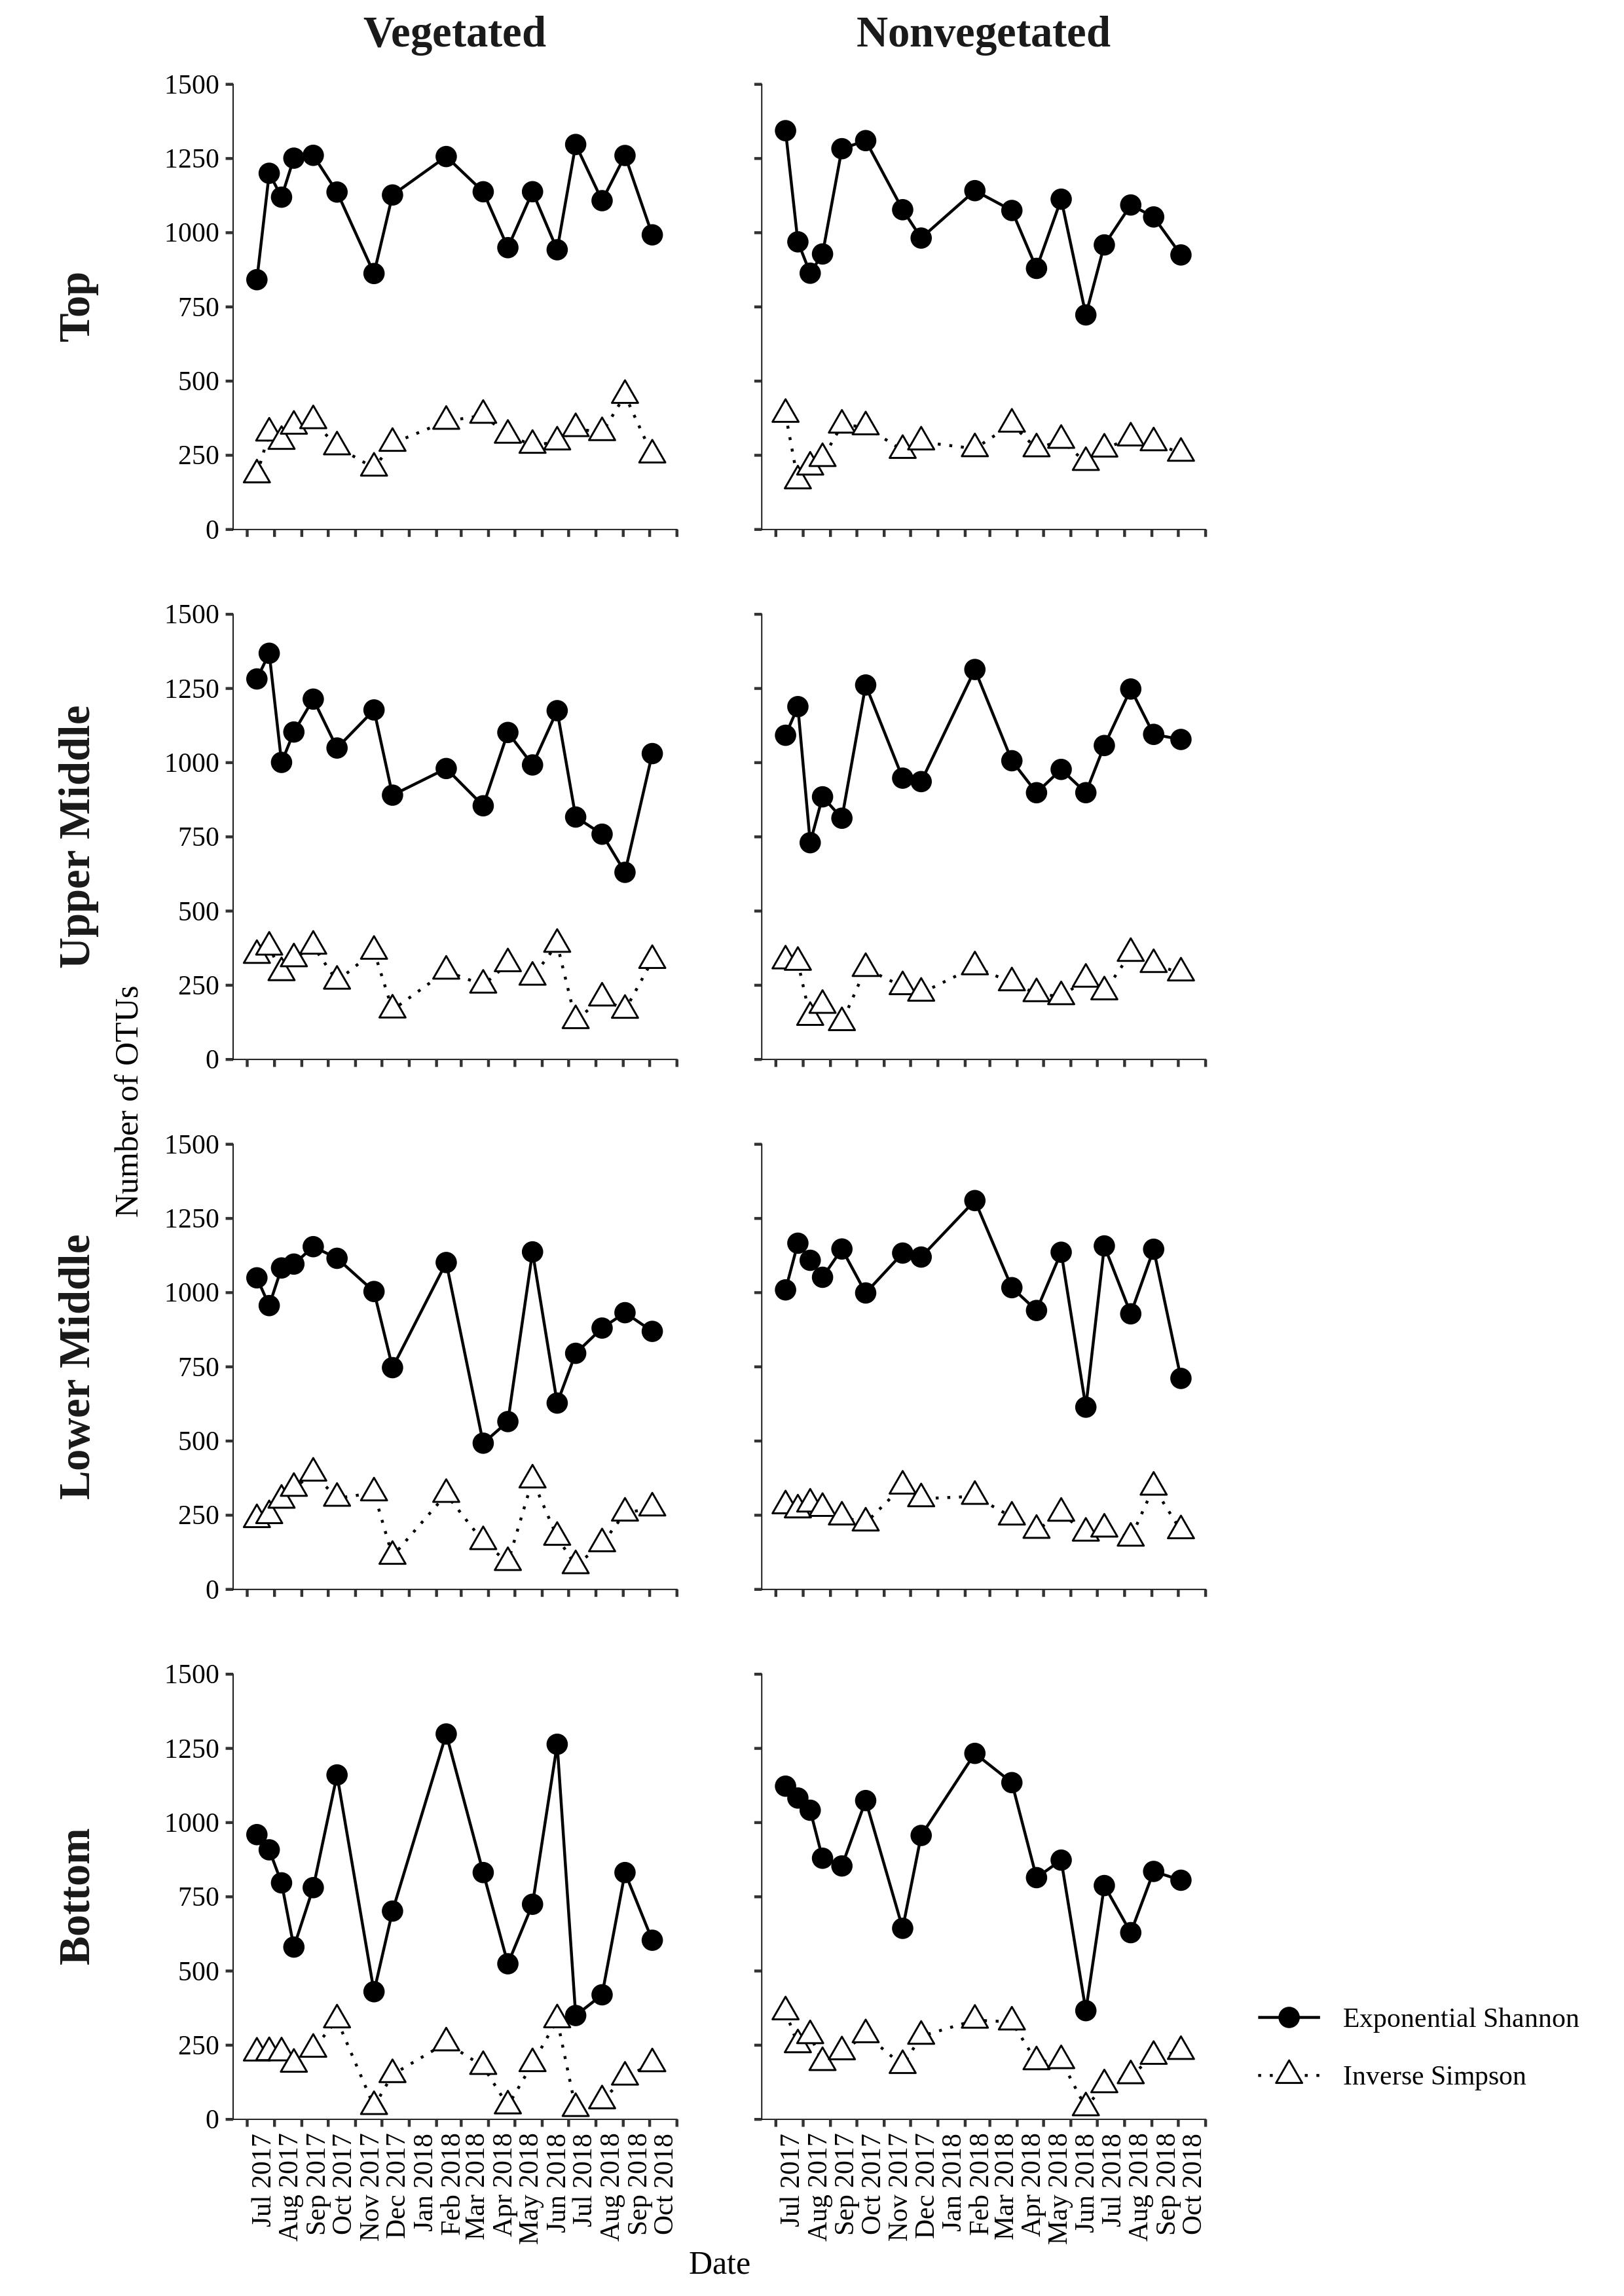
\includegraphics[width=0.9\linewidth,height=1\textheight]{../results/figures/diversity_indices_month} 

}

\caption{Temporal dynamics of the exponential Shannon diversity index and Inverse Simpson diversity index of sediment microbial communities sampled in different sediment layers of the vegetated and nonvegetated site in the Bay of Saline.\label{indices_moths}}\label{fig:unnamed-chunk-4}
\end{figure}

\begin{figure}[H]

{\centering 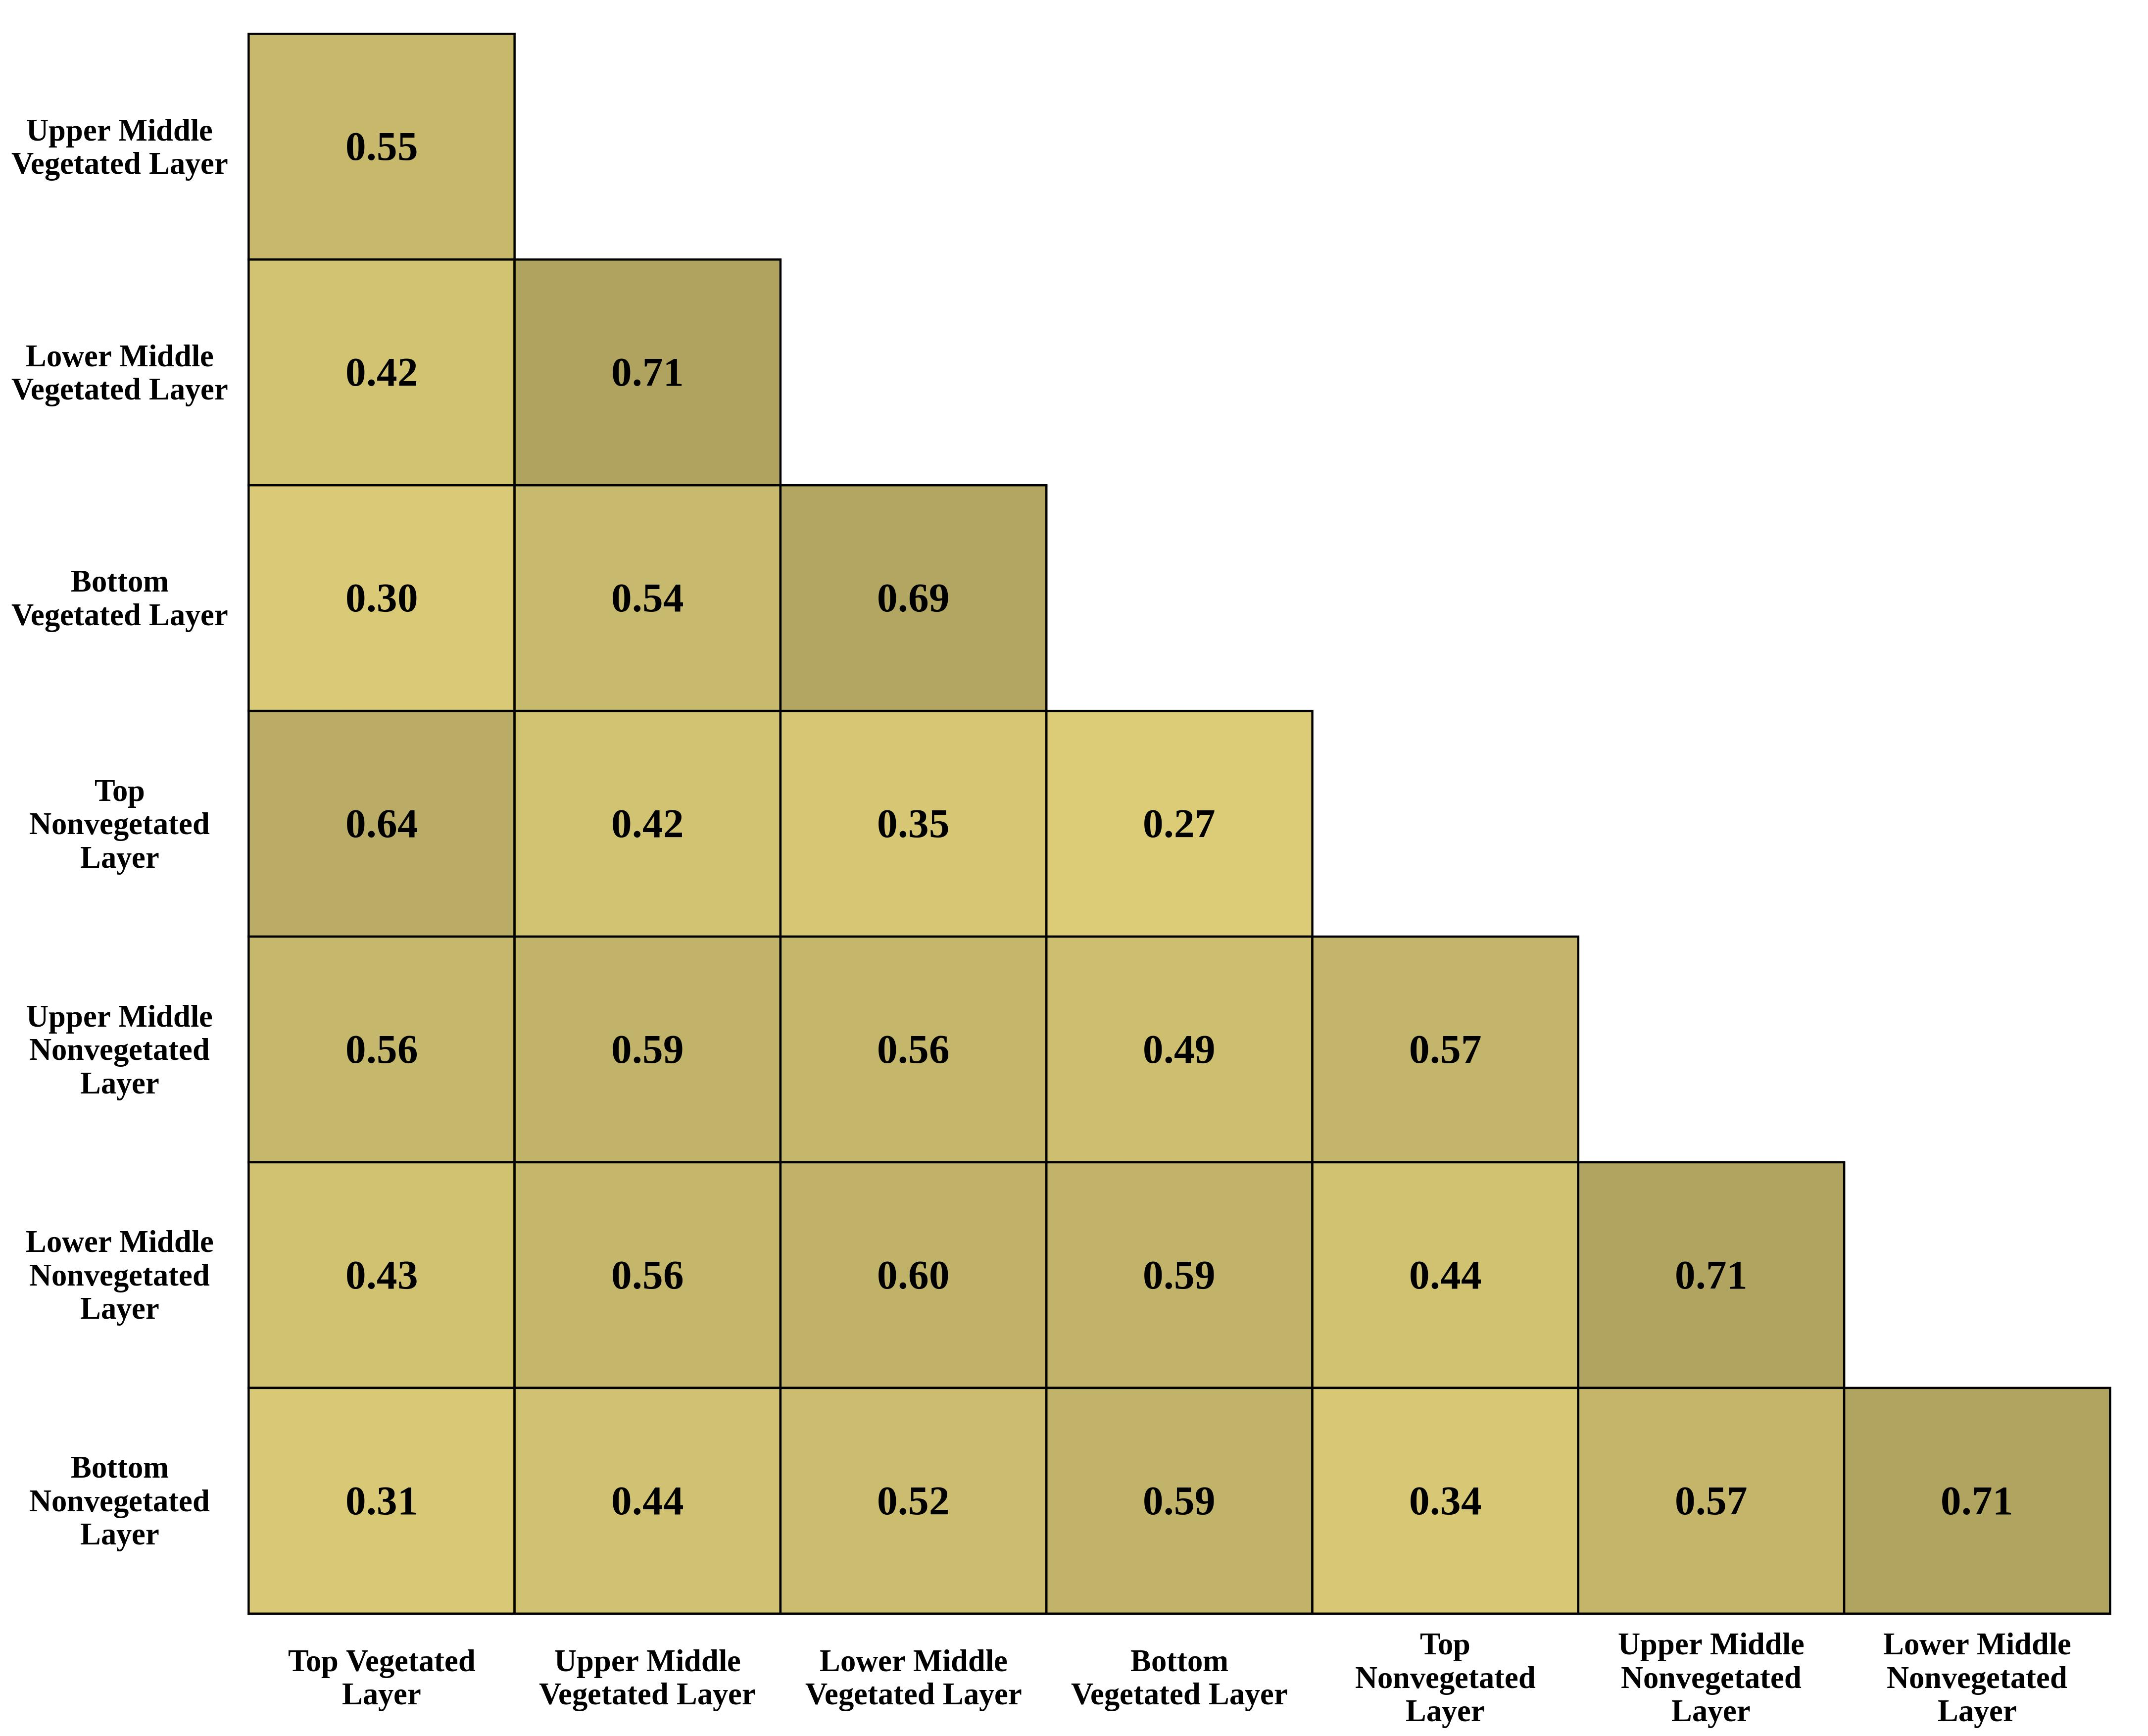
\includegraphics[width=1\linewidth,height=1\textheight]{../results/figures/matrix} 

}

\caption{Shared sediment microbial communities (Bray-Curtis similarity coefficient) between different sediment layers and sites in the Bay of Saline.\label{matrix}}\label{fig:unnamed-chunk-5}
\end{figure}

\begin{figure}[H]

{\centering 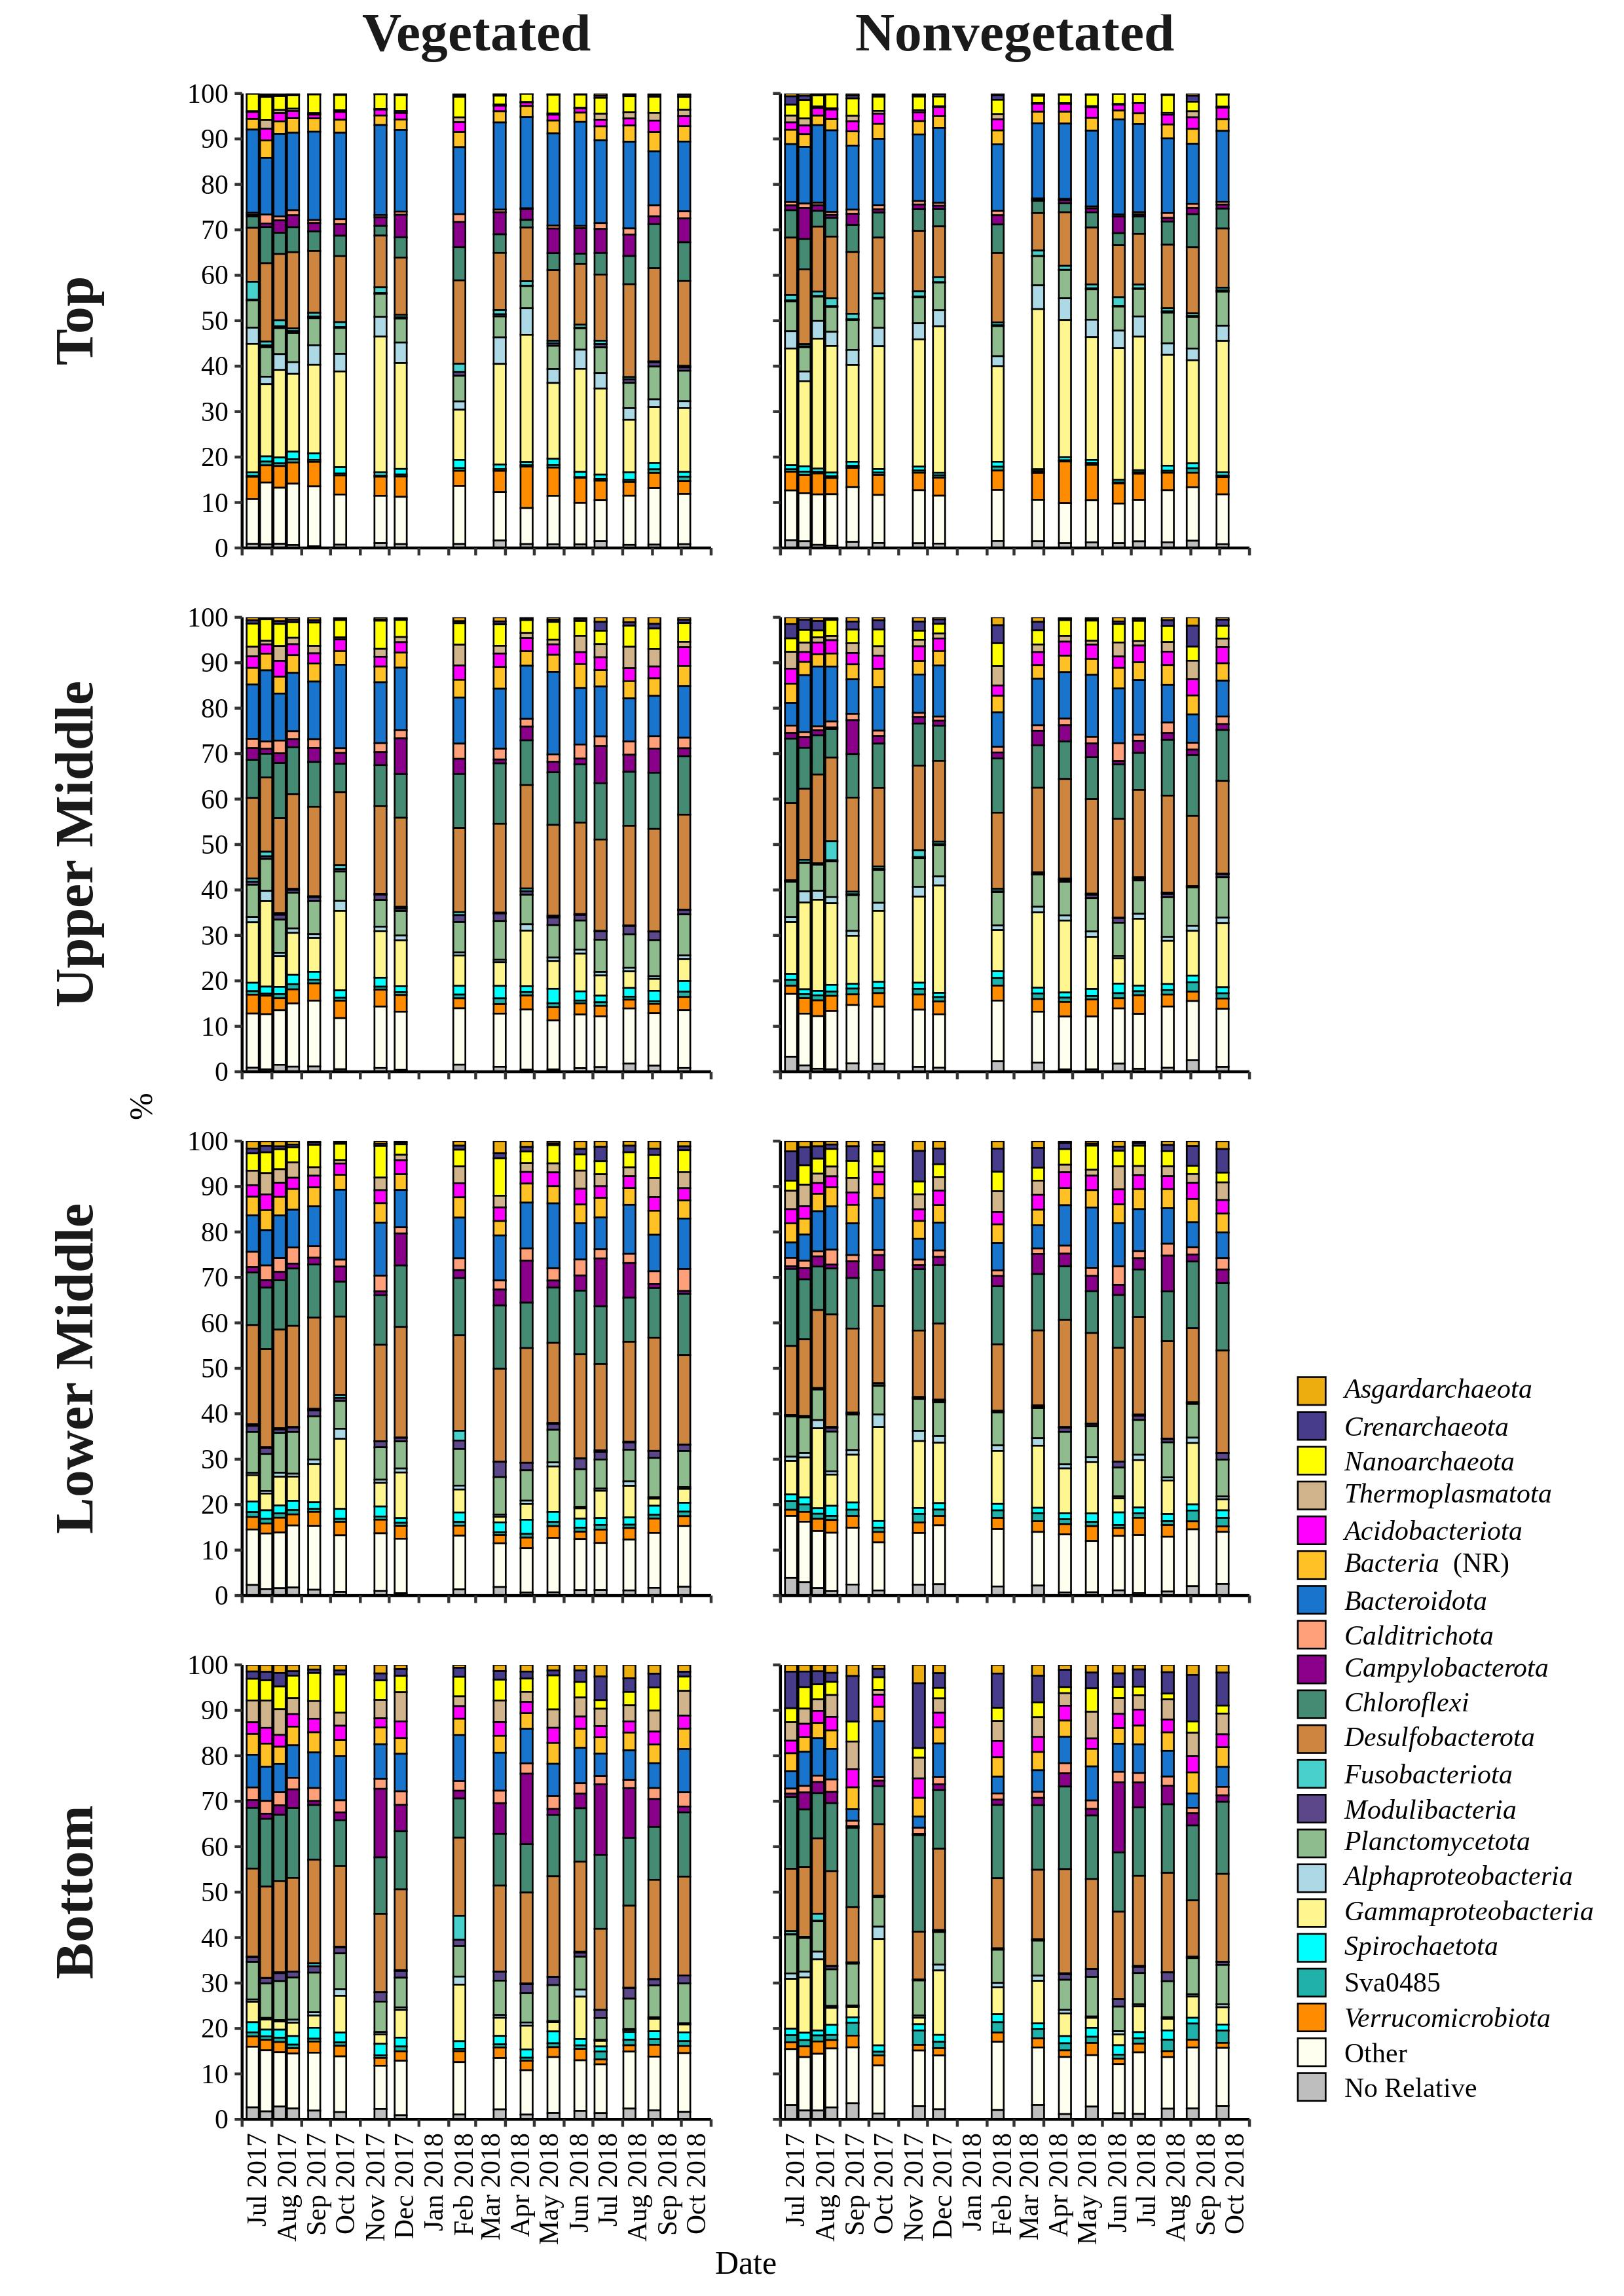
\includegraphics[width=1\linewidth,height=0.9\textheight]{../results/figures/community_barplot_month} 

}

\caption{Taxonomic classification and relative contribution of the most abundant bacterial and archaeal sequences ($\geq$ 3 \si{\percent}) of each sample taken in different sediment layers from the vegetated and nonvegetated site in the Bay of Saline. No Relative (NR) -- sequences without known relatives.\label{community_barplot_month}}\label{fig:unnamed-chunk-6}
\end{figure}

\newpage

\hypertarget{supplementary-tables}{%
\subsection{Supplementary tables}\label{supplementary-tables}}

\begingroup\fontsize{9}{11}\selectfont

\begin{longtable}[t]{cccccc}
\caption{\label{tab:nseq_notus}Sample ID, sampling date and site, sediment depth, no. of sequences and no. of OTUs of each sample. The number of sequences and OTUs was calculated after exclusion of sequences without known relatives (no relative sequences) and eukaryotic, chloroplast and mitochondrial sequences.\label{nseq_notus}}\\
\toprule
\textbf{Sample ID} & \textbf{Date} & \textbf{Site} & \textbf{Sediment Depth} & \textbf{No. of Sequences} & \textbf{No. of OTUs}\\
\midrule
\endfirsthead
\caption[]{Sample ID, sampling date and site, sediment depth, no. of sequences and no. of OTUs of each sample. The number of sequences and OTUs was calculated after exclusion of sequences without known relatives (no relative sequences) and eukaryotic, chloroplast and mitochondrial sequences.\label{nseq_notus} \textit{(continued)}}\\
\toprule
\textbf{Sample ID} & \textbf{Date} & \textbf{Site} & \textbf{Sediment Depth} & \textbf{No. of Sequences} & \textbf{No. of OTUs}\\
\midrule
\endhead

\endfoot
\bottomrule
\endlastfoot
76 & 12 July 2017 & Vegetated & 0 – 1 cm & 54,476 & 6,574\\
77 & 12 July 2017 & Vegetated & 2 – 3 cm & 55,381 & 7,608\\
78 & 12 July 2017 & Vegetated & 4 – 5 cm & 36,129 & 5,929\\
79 & 12 July 2017 & Vegetated & 7 – 8 cm & 48,135 & 6,590\\
80 & 12 July 2017 & Nonvegetated & 0 – 1 cm & 42,466 & 7,601\\
81 & 12 July 2017 & Nonvegetated & 2 – 3 cm & 13,568 & 3,210\\
82 & 12 July 2017 & Nonvegetated & 4 – 5 cm & 34,483 & 5,387\\
83 & 12 July 2017 & Nonvegetated & 7 – 8 cm & 21,281 & 4,147\\
96 & 26 July 2017 & Vegetated & 0 – 1 cm & 14,141 & 4,126\\
97 & 26 July 2017 & Vegetated & 1 – 2 cm & 13,607 & 4,434\\
98 & 26 July 2017 & Vegetated & 4 – 5 cm & 13,686 & 3,396\\
99 & 26 July 2017 & Vegetated & 7 – 8 cm & 13,558 & 3,352\\
100 & 26 July 2017 & Nonvegetated & 0 – 1 cm & 15,116 & 4,113\\
101 & 26 July 2017 & Nonvegetated & 1 – 2 cm & 14,701 & 4,318\\
102 & 26 July 2017 & Nonvegetated & 4 – 5 cm & 14,012 & 4,080\\
103 & 26 July 2017 & Nonvegetated & 7 – 8 cm & 14,494 & 4,158\\
116 & 9 August 2017 & Vegetated & 0 – 1 cm & 30,722 & 4,894\\
117 & 9 August 2017 & Vegetated & 2 – 3 cm & 27,363 & 4,141\\
118 & 9 August 2017 & Vegetated & 4 – 5 cm & 24,476 & 4,405\\
119 & 9 August 2017 & Vegetated & 7 – 8 cm & 27,941 & 3,691\\
120 & 9 August 2017 & Nonvegetated & 0 – 1 cm & 27,645 & 4,152\\
121 & 9 August 2017 & Nonvegetated & 2 – 3 cm & 30,154 & 3,929\\
122 & 9 August 2017 & Nonvegetated & 4 – 5 cm & 29,084 & 4,816\\
123 & 9 August 2017 & Nonvegetated & 7 – 8 cm & 30,128 & 4,787\\
136 & 23 August 2017 & Vegetated & 0 – 1 cm & 29,381 & 5,541\\
137 & 23 August 2017 & Vegetated & 2 – 3 cm & 38,507 & 5,391\\
138 & 23 August 2017 & Vegetated & 4 – 5 cm & 26,101 & 4,896\\
139 & 23 August 2017 & Vegetated & 7 – 8 cm & 17,524 & 2,388\\
140 & 23 August 2017 & Nonvegetated & 0 – 1 cm & 41,344 & 5,663\\
141 & 23 August 2017 & Nonvegetated & 2 – 3 cm & 35,724 & 5,361\\
142 & 23 August 2017 & Nonvegetated & 4 – 5 cm & 26,572 & 4,919\\
143 & 23 August 2017 & Nonvegetated & 7 – 8 cm & 26,310 & 4,385\\
156 & 14 September 2017 & Vegetated & 0 – 1 cm & 35,609 & 5,541\\
157 & 14 September 2017 & Vegetated & 2 – 3 cm & 38,113 & 5,249\\
158 & 14 September 2017 & Vegetated & 4 – 5 cm & 27,996 & 4,606\\
159 & 14 September 2017 & Vegetated & 7 – 8 cm & 31,834 & 3,750\\
160 & 14 September 2017 & Nonvegetated & 0 – 1 cm & 33,666 & 5,487\\
161 & 14 September 2017 & Nonvegetated & 2 – 3 cm & 28,251 & 4,174\\
162 & 14 September 2017 & Nonvegetated & 4 – 5 cm & 27,073 & 4,830\\
163 & 14 September 2017 & Nonvegetated & 7 – 8 cm & 31,422 & 4,316\\
176 & 11 October 2017 & Vegetated & 0 – 1 cm & 16,751 & 4,653\\
177 & 11 October 2017 & Vegetated & 2 – 3 cm & 15,991 & 4,292\\
178 & 11 October 2017 & Vegetated & 3 – 4 cm & 15,385 & 4,191\\
179 & 11 October 2017 & Vegetated & 7 – 8 cm & 16,641 & 4,300\\
180 & 11 October 2017 & Nonvegetated & 0 – 1 cm & 9,722 & 3,576\\
181 & 11 October 2017 & Nonvegetated & 2 – 3 cm & 12,470 & 4,038\\
182 & 11 October 2017 & Nonvegetated & 3 – 4 cm & 17,612 & 4,486\\
183 & 11 October 2017 & Nonvegetated & 7 – 8 cm & 17,080 & 4,514\\
196 & 22 November 2017 & Vegetated & 0 – 1 cm & 26,747 & 4,023\\
197 & 22 November 2017 & Vegetated & 2 – 3 cm & 26,663 & 4,429\\
198 & 22 November 2017 & Vegetated & 4 – 5 cm & 27,062 & 4,200\\
199 & 22 November 2017 & Vegetated & 7 – 8 cm & 29,368 & 3,280\\
200 & 22 November 2017 & Nonvegetated & 0 – 1 cm & 33,555 & 5,271\\
201 & 22 November 2017 & Nonvegetated & 2 – 3 cm & 24,602 & 3,898\\
202 & 22 November 2017 & Nonvegetated & 4 – 5 cm & 22,820 & 4,398\\
203 & 22 November 2017 & Nonvegetated & 7 – 8 cm & 21,685 & 3,046\\
216 & 13 December 2017 & Vegetated & 0 – 1 cm & 29,217 & 4,742\\
217 & 13 December 2017 & Vegetated & 2 – 3 cm & 22,379 & 3,630\\
218 & 13 December 2017 & Vegetated & 4 – 5 cm & 27,460 & 3,948\\
219 & 13 December 2017 & Vegetated & 7 – 8 cm & 33,757 & 3,994\\
220 & 13 December 2017 & Nonvegetated & 0 – 1 cm & 30,110 & 4,634\\
221 & 13 December 2017 & Nonvegetated & 2 – 3 cm & 35,557 & 4,921\\
222 & 13 December 2017 & Nonvegetated & 4 – 5 cm & 31,732 & 4,784\\
223 & 13 December 2017 & Nonvegetated & 7 – 8 cm & 26,860 & 3,988\\
236 & 12 February 2018 & Vegetated & 0 – 1 cm & 12,249 & 3,778\\
237 & 12 February 2018 & Vegetated & 2 – 3 cm & 13,328 & 3,364\\
238 & 12 February 2018 & Vegetated & 4 – 5 cm & 11,317 & 3,449\\
239 & 12 February 2018 & Vegetated & 7 – 8 cm & 14,574 & 4,518\\
240 & 12 February 2018 & Nonvegetated & 0 – 1 cm & 13,730 & 4,146\\
241 & 12 February 2018 & Nonvegetated & 2 – 3 cm & 14,416 & 4,590\\
242 & 12 February 2018 & Nonvegetated & 4 – 5 cm & 13,317 & 4,423\\
243 & 12 February 2018 & Nonvegetated & 7 – 8 cm & 21,480 & 5,363\\
256 & 26 March 2018 & Vegetated & 0 – 1 cm & 28,906 & 4,313\\
257 & 26 March 2018 & Vegetated & 2 – 3 cm & 19,307 & 2,911\\
258 & 26 March 2018 & Vegetated & 5 – 6 cm & 22,957 & 2,444\\
259 & 26 March 2018 & Vegetated & 7 – 8 cm & 31,090 & 4,270\\
260 & 26 March 2018 & Nonvegetated & 0 – 1 cm & 30,528 & 4,579\\
261 & 26 March 2018 & Nonvegetated & 2 – 3 cm & 36,972 & 5,142\\
262 & 26 March 2018 & Nonvegetated & 5 – 6 cm & 38,650 & 5,522\\
263 & 26 March 2018 & Nonvegetated & 7 – 8 cm & 24,660 & 4,834\\
276 & 23 April 2018 & Vegetated & 0 – 1 cm & 25,010 & 3,714\\
277 & 23 April 2018 & Vegetated & 2 – 3 cm & 35,406 & 4,712\\
278 & 23 April 2018 & Vegetated & 4 – 5 cm & 35,154 & 4,008\\
279 & 23 April 2018 & Vegetated & 7 – 8 cm & 26,658 & 3,965\\
280 & 23 April 2018 & Nonvegetated & 0 – 1 cm & 30,854 & 4,055\\
281 & 23 April 2018 & Nonvegetated & 2 – 3 cm & 33,005 & 4,742\\
282 & 23 April 2018 & Nonvegetated & 4 – 5 cm & 37,048 & 5,017\\
283 & 23 April 2018 & Nonvegetated & 7 – 8 cm & 16,686 & 3,271\\
296 & 21 May 2018 & Vegetated & 0 – 1 cm & 14,063 & 4,009\\
297 & 21 May 2018 & Vegetated & 2 – 3 cm & 13,148 & 3,441\\
298 & 21 May 2018 & Vegetated & 3 – 4 cm & 13,120 & 3,553\\
299 & 21 May 2018 & Vegetated & 7 – 8 cm & 14,266 & 3,050\\
300 & 21 May 2018 & Nonvegetated & 0 – 1 cm & 10,825 & 3,462\\
301 & 21 May 2018 & Nonvegetated & 2 – 3 cm & 13,392 & 3,750\\
302 & 21 May 2018 & Nonvegetated & 3 – 4 cm & 10,768 & 3,541\\
303 & 21 May 2018 & Nonvegetated & 7 – 8 cm & 13,103 & 3,471\\
316 & 18 June 2018 & Vegetated & 0 – 1 cm & 22,280 & 3,874\\
317 & 18 June 2018 & Vegetated & 2 – 3 cm & 18,356 & 3,602\\
318 & 18 June 2018 & Vegetated & 4 – 5 cm & 28,066 & 3,309\\
319 & 18 June 2018 & Vegetated & 7 – 8 cm & 30,028 & 5,217\\
320 & 18 June 2018 & Nonvegetated & 0 – 1 cm & 32,190 & 3,929\\
321 & 18 June 2018 & Nonvegetated & 2 – 3 cm & 22,167 & 3,797\\
322 & 18 June 2018 & Nonvegetated & 4 – 5 cm & 30,626 & 3,264\\
323 & 18 June 2018 & Nonvegetated & 7 – 8 cm & 30,259 & 3,071\\
336 & 9 July 2018 & Vegetated & 0 – 1 cm & 11,589 & 3,844\\
337 & 9 July 2018 & Vegetated & 2 – 3 cm & 14,299 & 3,690\\
338 & 9 July 2018 & Vegetated & 4 – 5 cm & 10,031 & 3,276\\
339 & 9 July 2018 & Vegetated & 7 – 8 cm & 13,117 & 2,521\\
340 & 9 July 2018 & Nonvegetated & 0 – 1 cm & 13,328 & 3,425\\
341 & 9 July 2018 & Nonvegetated & 2 – 3 cm & 12,897 & 3,926\\
342 & 9 July 2018 & Nonvegetated & 4 – 5 cm & 11,252 & 3,822\\
343 & 9 July 2018 & Nonvegetated & 7 – 8 cm & 11,902 & 3,211\\
356 & 8 August 2018 & Vegetated & 0 – 1 cm & 24,862 & 4,654\\
357 & 8 August 2018 & Vegetated & 2 – 3 cm & 28,104 & 3,584\\
358 & 8 August 2018 & Vegetated & 4 – 5 cm & 23,108 & 4,125\\
359 & 8 August 2018 & Vegetated & 7 – 8 cm & 24,151 & 2,782\\
360 & 8 August 2018 & Nonvegetated & 0 – 1 cm & 25,781 & 4,741\\
361 & 8 August 2018 & Nonvegetated & 2 – 3 cm & 29,308 & 4,822\\
362 & 8 August 2018 & Nonvegetated & 4 – 5 cm & 29,364 & 4,649\\
363 & 8 August 2018 & Nonvegetated & 7 – 8 cm & 26,580 & 3,422\\
376 & 3 September 2018 & Vegetated & 0 – 1 cm & 26,186 & 4,632\\
377 & 3 September 2018 & Vegetated & 2 – 3 cm & 27,575 & 3,337\\
378 & 3 September 2018 & Vegetated & 4 – 5 cm & 28,887 & 4,249\\
379 & 3 September 2018 & Vegetated & 7 – 8 cm & 25,855 & 4,184\\
380 & 3 September 2018 & Nonvegetated & 0 – 1 cm & 14,868 & 3,481\\
381 & 3 September 2018 & Nonvegetated & 2 – 3 cm & 26,415 & 4,443\\
382 & 3 September 2018 & Nonvegetated & 4 – 5 cm & 11,945 & 3,010\\
383 & 3 September 2018 & Nonvegetated & 7 – 8 cm & 25,845 & 3,993\\
396 & 4 October 2018 & Vegetated & 0 – 1 cm & 20,085 & 3,933\\
397 & 4 October 2018 & Vegetated & 2 – 3 cm & 35,809 & 4,306\\
398 & 4 October 2018 & Vegetated & 4 – 5 cm & 28,130 & 3,692\\
399 & 4 October 2018 & Vegetated & 7 – 8 cm & 26,114 & 2,845\\
400 & 4 October 2018 & Nonvegetated & 0 – 1 cm & 27,823 & 4,307\\
401 & 4 October 2018 & Nonvegetated & 2 – 3 cm & 32,430 & 4,796\\
402 & 4 October 2018 & Nonvegetated & 4 – 5 cm & 28,865 & 3,645\\
403 & 4 October 2018 & Nonvegetated & 7 – 8 cm & 26,764 & 3,695\\*
\end{longtable}
\endgroup{}

\begingroup\fontsize{9}{11}\selectfont

\begin{longtable}[t]{>{\centering\arraybackslash}m{8.5em}>{\centering\arraybackslash}m{4em}>{\centering\arraybackslash}m{4em}>{\centering\arraybackslash}m{4em}>{\centering\arraybackslash}m{20em}>{\centering\arraybackslash}m{4em}}
\caption{\label{tab:estimators}Statistic of richness estimator and diversity index parameters of sediment microbial communities sampled in different sediment layers of the vegetated site in the Bay of Saline. Parameters were tested by applying the Kruskal-Wallis \textit{H} test followed by a pairwise comparison using the Mann-Whitney \textit{U} test. Bonferroni correction was used to address the problem of multiple comparisons.\label{calculator_statistics}}\\
\toprule
\multicolumn{1}{c}{\textbf{ }} & \multicolumn{3}{c}{\textbf{Kruskal-Wallis \textit{H} test}} & \multicolumn{2}{c}{\textbf{Mann-Whitney \textit{U} test}} \\
\cmidrule(l{3pt}r{3pt}){2-4} \cmidrule(l{3pt}r{3pt}){5-6}
\textbf{Parameter} & \textbf{\textit{H}} & \textbf{\textit{df}} & \textbf{\textit{p}} & \textbf{Comparisons Between Sediment Layers} & \textbf{\textit{p}}\\
\midrule
\endfirsthead
\caption[]{Statistic of richness estimator and diversity index parameters of sediment microbial communities sampled in different sediment layers of the vegetated site in the Bay of Saline. Parameters were tested by applying the Kruskal-Wallis \textit{H} test followed by a pairwise comparison using the Mann-Whitney \textit{U} test. Bonferroni correction was used to address the problem of multiple comparisons.\label{calculator_statistics} \textit{(continued)}}\\
\toprule
\multicolumn{1}{c}{\textbf{ }} & \multicolumn{3}{c}{\textbf{Kruskal-Wallis \textit{H} test}} & \multicolumn{2}{c}{\textbf{Mann-Whitney \textit{U} test}} \\
\cmidrule(l{3pt}r{3pt}){2-4} \cmidrule(l{3pt}r{3pt}){5-6}
\textbf{Parameter} & \textbf{\textit{H}} & \textbf{\textit{df}} & \textbf{\textit{p}} & \textbf{Comparisons Between Sediment Layers} & \textbf{\textit{p}}\\
\midrule
\endhead

\endfoot
\bottomrule
\endlastfoot
 & &  &  & Top Layer – Upper Middle Layer & 0.78\\
\nopagebreak
 & &  &  & Top Layer – Lower Middle Layer & 0.38\\
\nopagebreak
 & &  &  & Top Layer – Bottom Layer & < 0.05\\
\nopagebreak
 & &  &  & Upper Middle Layer – Lower Middle Layer & 1.00\\
\nopagebreak
 & &  &  & Upper Middle Layer – Bottom Layer & 0.21\\
\nopagebreak
\multirow{-6}{8.5em}{\centering\arraybackslash Observed No. of OTUs} & \multirow{-6}{*}{\centering\arraybackslash 11.5 } & \multirow{-6}{*}{\centering\arraybackslash 3 } & \multirow{-6}{*}{\centering\arraybackslash < 0.01 } & Lower Middle Layer – Bottom Layer & 0.63\\
\cmidrule{1-6}\pagebreak[0]
 & &  &  & Top Layer – Upper Middle Layer & 1.00\\
\nopagebreak
 & &  &  & Top Layer – Lower Middle Layer & 1.00\\
\nopagebreak
 & &  &  & Top Layer – Bottom Layer & 0.23\\
\nopagebreak
 & &  &  & Upper Middle Layer – Lower Middle Layer & 1.00\\
\nopagebreak
 & &  &  & Upper Middle Layer – Bottom Layer & 1.00\\
\nopagebreak
\multirow{-6}{8.5em}{\centering\arraybackslash Chao1} & \multirow{-6}{*}{\centering\arraybackslash 4.7 } & \multirow{-6}{*}{\centering\arraybackslash 3 } & \multirow{-6}{*}{\centering\arraybackslash 0.20 } & Lower Middle Layer – Bottom Layer & 1.00\\
\cmidrule{1-6}\pagebreak[0]
 & &  &  & Top Layer – Upper Middle Layer & 0.78\\
\nopagebreak
 & &  &  & Top Layer – Lower Middle Layer & 1.00\\
\nopagebreak
 & &  &  & Top Layer – Bottom Layer & 0.15\\
\nopagebreak
 & &  &  & Upper Middle Layer – Lower Middle Layer & 1.00\\
\nopagebreak
 & &  &  & Upper Middle Layer – Bottom Layer & 1.00\\
\nopagebreak
\multirow{-6}{8.5em}{\centering\arraybackslash ACE} & \multirow{-6}{*}{\centering\arraybackslash 5.7 } & \multirow{-6}{*}{\centering\arraybackslash 3 } & \multirow{-6}{*}{\centering\arraybackslash 0.13 } & Lower Middle Layer – Bottom Layer & 1.00\\
\cmidrule{1-6}\pagebreak[0]
 & &  &  & Top Layer – Upper Middle Layer & 0.95\\
\nopagebreak
 & &  &  & Top Layer – Lower Middle Layer & < 0.05\\
\nopagebreak
 & &  &  & Top Layer – Bottom Layer & < 0.01\\
\nopagebreak
 & &  &  & Upper Middle Layer – Lower Middle Layer & 1.00\\
\nopagebreak
 & &  &  & Upper Middle Layer – Bottom Layer & < 0.05\\
\nopagebreak
\multirow{-6}{8.5em}{\centering\arraybackslash Exponential Shannon} & \multirow{-6}{*}{\centering\arraybackslash 16.4 } & \multirow{-6}{*}{\centering\arraybackslash 3 } & \multirow{-6}{*}{\centering\arraybackslash < 0.001 } & Lower Middle Layer – Bottom Layer & 0.63\\
\cmidrule{1-6}\pagebreak[0]
 & &  &  & Top Layer – Upper Middle Layer & 1.00\\
\nopagebreak
 & &  &  & Top Layer – Lower Middle Layer & 0.32\\
\nopagebreak
 & &  &  & Top Layer – Bottom Layer & < 0.01\\
\nopagebreak
 & &  &  & Upper Middle Layer – Lower Middle Layer & 1.00\\
\nopagebreak
 & &  &  & Upper Middle Layer – Bottom Layer & < 0.05\\
\nopagebreak
\multirow{-6}{8.5em}{\centering\arraybackslash Inverse Simpson} & \multirow{-6}{*}{\centering\arraybackslash 16.4 } & \multirow{-6}{*}{\centering\arraybackslash 3 } & \multirow{-6}{*}{\centering\arraybackslash < 0.001 } & Lower Middle Layer – Bottom Layer & 0.44\\*
\end{longtable}
\endgroup{}

\newpage

\begingroup\fontsize{9}{11}\selectfont

\begin{longtable}[t]{>{\centering\arraybackslash}m{10.5em}>{\centering\arraybackslash}m{3em}>{\centering\arraybackslash}m{3em}>{\centering\arraybackslash}m{3em}>{\centering\arraybackslash}m{22em}>{\centering\arraybackslash}m{3em}}
\caption{\label{tab:estimators}Statistic of richness estimator and diversity index parameters of sediment microbial communities sampled in different sediment layers of the nonvegetated site in the Bay of Saline. Parameters were tested by applying the Kruskal-Wallis \textit{H} test followed by a pairwise comparison using the Mann-Whitney \textit{U} test. Bonferroni correction was used to address the problem of multiple comparisons.\label{calculator_statisticsN}}\\
\toprule
\multicolumn{1}{c}{\textbf{ }} & \multicolumn{3}{c}{\textbf{Kruskal-Wallis \textit{H} test}} & \multicolumn{2}{c}{\textbf{Mann-Whitney \textit{U} test}} \\
\cmidrule(l{3pt}r{3pt}){2-4} \cmidrule(l{3pt}r{3pt}){5-6}
\textbf{Parameter} & \textbf{\textit{H}} & \textbf{\textit{df}} & \textbf{\textit{p}} & \textbf{Comparisons Between Sediment Layers} & \textbf{\textit{p}}\\
\midrule
\endfirsthead
\caption[]{Statistic of richness estimator and diversity index parameters of sediment microbial communities sampled in different sediment layers of the nonvegetated site in the Bay of Saline. Parameters were tested by applying the Kruskal-Wallis \textit{H} test followed by a pairwise comparison using the Mann-Whitney \textit{U} test. Bonferroni correction was used to address the problem of multiple comparisons.\label{calculator_statisticsN} \textit{(continued)}}\\
\toprule
\multicolumn{1}{c}{\textbf{ }} & \multicolumn{3}{c}{\textbf{Kruskal-Wallis \textit{H} test}} & \multicolumn{2}{c}{\textbf{Mann-Whitney \textit{U} test}} \\
\cmidrule(l{3pt}r{3pt}){2-4} \cmidrule(l{3pt}r{3pt}){5-6}
\textbf{Parameter} & \textbf{\textit{H}} & \textbf{\textit{df}} & \textbf{\textit{p}} & \textbf{Comparisons Between Sediment Layers} & \textbf{\textit{p}}\\
\midrule
\endhead

\endfoot
\bottomrule
\endlastfoot
 & &  &  & Top Layer – Upper Middle Layer & 1.00\\
\nopagebreak
 & &  &  & Top Layer – Lower Middle Layer & 1.00\\
\nopagebreak
 & &  &  & Top Layer – Bottom Layer & 0.59\\
\nopagebreak
 & &  &  & Upper Middle Layer – Lower Middle Layer & 1.00\\
\nopagebreak
 & &  &  & Upper Middle Layer – Bottom Layer & 0.89\\
\nopagebreak
\multirow{-6}{10.5em}{\centering\arraybackslash Observed No. of OTUs} & \multirow{-6}{*}{\centering\arraybackslash 5.1 } & \multirow{-6}{*}{\centering\arraybackslash 3 } & \multirow{-6}{*}{\centering\arraybackslash 0.16 } & Lower Middle Layer – Bottom Layer & 0.27\\
\cmidrule{1-6}\pagebreak[0]
 & &  &  & Top Layer – Upper Middle Layer & 1.00\\
\nopagebreak
 & &  &  & Top Layer – Lower Middle Layer & 1.00\\
\nopagebreak
 & &  &  & Top Layer – Bottom Layer & 0.51\\
\nopagebreak
 & &  &  & Upper Middle Layer – Lower Middle Layer & 1.00\\
\nopagebreak
 & &  &  & Upper Middle Layer – Bottom Layer & 1.00\\
\nopagebreak
\multirow{-6}{10.5em}{\centering\arraybackslash Chao1} & \multirow{-6}{*}{\centering\arraybackslash 3.7 } & \multirow{-6}{*}{\centering\arraybackslash 3 } & \multirow{-6}{*}{\centering\arraybackslash 0.30 } & Lower Middle Layer – Bottom Layer & 0.95\\
\cmidrule{1-6}\pagebreak[0]
 & &  &  & Top Layer – Upper Middle Layer & 1.00\\
\nopagebreak
 & &  &  & Top Layer – Lower Middle Layer & 1.00\\
\nopagebreak
 & &  &  & Top Layer – Bottom Layer & 0.44\\
\nopagebreak
 & &  &  & Upper Middle Layer – Lower Middle Layer & 1.00\\
\nopagebreak
 & &  &  & Upper Middle Layer – Bottom Layer & 1.00\\
\nopagebreak
\multirow{-6}{10.5em}{\centering\arraybackslash ACE} & \multirow{-6}{*}{\centering\arraybackslash 4.1 } & \multirow{-6}{*}{\centering\arraybackslash 3 } & \multirow{-6}{*}{\centering\arraybackslash 0.26 } & Lower Middle Layer – Bottom Layer & 0.95\\
\cmidrule{1-6}\pagebreak[0]
 & &  &  & Top Layer – Upper Middle Layer & 1.00\\
\nopagebreak
 & &  &  & Top Layer – Lower Middle Layer & 1.00\\
\nopagebreak
 & &  &  & Top Layer – Bottom Layer & 0.21\\
\nopagebreak
 & &  &  & Upper Middle Layer – Lower Middle Layer & 1.00\\
\nopagebreak
 & &  &  & Upper Middle Layer – Bottom Layer & 0.35\\
\nopagebreak
\multirow{-6}{10.5em}{\centering\arraybackslash Exponential Shannon} & \multirow{-6}{*}{\centering\arraybackslash 7.1 } & \multirow{-6}{*}{\centering\arraybackslash 3 } & \multirow{-6}{*}{\centering\arraybackslash 0.07 } & Lower Middle Layer – Bottom Layer & 0.16\\
\cmidrule{1-6}\pagebreak[0]
 & &  &  & Top Layer – Upper Middle Layer & 1.00\\
\nopagebreak
 & &  &  & Top Layer – Lower Middle Layer & 1.00\\
\nopagebreak
 & &  &  & Top Layer – Bottom Layer & 0.25\\
\nopagebreak
 & &  &  & Upper Middle Layer – Lower Middle Layer & 1.00\\
\nopagebreak
 & &  &  & Upper Middle Layer – Bottom Layer & 1.00\\
\nopagebreak
\multirow{-6}{10.5em}{\centering\arraybackslash Inverse Simpson} & \multirow{-6}{*}{\centering\arraybackslash 4.7 } & \multirow{-6}{*}{\centering\arraybackslash 3 } & \multirow{-6}{*}{\centering\arraybackslash 0.20 } & Lower Middle Layer – Bottom Layer & 1.00\\*
\end{longtable}
\endgroup{}

\end{document}
